\chapter{Diseño de Hardware}

\section{Diagrama en Bloques}

\subsection{Recepción Inalámbrica}

\paragraph{}
Para implementar el manejo por control remoto se utiliza el protocolo Bluetooth, 
más especificamente el módulo HM-10, que funciona como una comunicación serie
inalámbrica. Del lado del usuario se utiliza la aplicación de Android
"BLEJoystick", disponible en Google Play Store. También se cuenta con un LED
para indicar la correcta vinculacion entre la app y el módulo bluetooth.

\subsubsection{Componentes a Utilizar}

\begin{longtable}[]{|c|c|c|c|p{3.2cm}|c|}
	\toprule
	Componente & Código & Valor & Cantidad & Función &
	Protocolo\tabularnewline
	\midrule
	\endhead
	Rx/Tx BLE & HM-10 & - & 1 & Recepción & UART
	8N1\tabularnewline
	LED & - & Rojo 3mm & 1 & Informar estado\newline de la conexión Bluetooth &
	Digital\tabularnewline
	\bottomrule
\end{longtable}

\subsubsection{Rx/Tx BLE}

\begin{figure}[H]
	\centering
	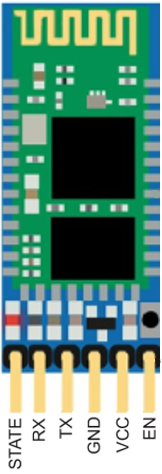
\includegraphics[width=0.15\linewidth]{informe_2/encapsulado_HM-10}
	\caption{HM-10}
	\label{fig:encapsuladohm-10}
\end{figure}


\paragraph{}El módulo Bluetooth a utilizar es el HM-10 provisto por la cátedra, el cual ya
fue utilizado en asignaturas anteriores por lo cual se conocen sus características 
y su funcionamiento.
Además, la sAPI de la CIAA provee una librería para comunicación Bluetooth, facilitando 
su programación.

\paragraph{}Respecto a las características de Hardware, el HM-10 funciona a 3.3v, por lo que
no hay que realizar ninguna adaptación para su funcionamiento.

\subsubsection{LED}

\paragraph{}Para la alimentación del LED se utiliza el puerto GPIO1, realizando los 
siguientes cálculos se obtiene el valor de la resistencia que necesita 
para su conexión::


$$ \mathrm{R} = \frac{\mathrm{V} - \mathrm{LED_V}}{\mathrm{LED_I}} = 420\Omega $$

$ \mathrm{V} = 3.3\mathrm{v};\ \mathrm{LED_V} = 1.2\mathrm{v};\ \mathrm{LED_I} = 5\mathrm{mA};  $

\subsubsection{Conexionado}

\paragraph{HM-10} El módulo Bluetooth se comunica a través de un protocolo serie 8N1,
a 9600 bps, y se configura a través de comandos AT. Las librerías de la CIAA
ya proveen funciones para establecer una comunicación con un módulo HM-10.

\paragraph{LED}Se conecta de manera directa a una salida digital del integrado, 
teniendo en cuenta la resistencia mencionada.

\subsubsection{Esquemático}

\begin{figure}[H]
	\centering
	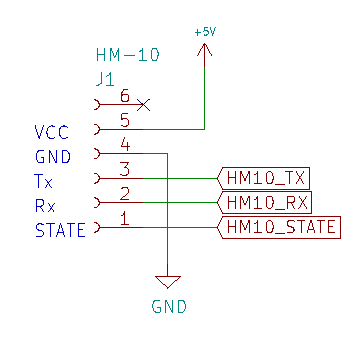
\includegraphics[width=0.5\linewidth]{informe_3/schem_hm10}
	\caption{Conexionado del Módulo Bluetooth HM-10}
	\label{fig:schemhm10}
\end{figure}

\begin{figure}[H]
	\centering
	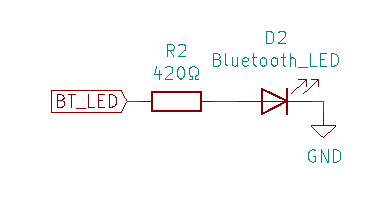
\includegraphics[width=0.5\linewidth]{informe_3/schem_bt_led}
	\caption{Conexionado del LED Bluetooth}
	\label{fig:schemledbt}
\end{figure}

\subsection{Controlador de Motores}

\paragraph{}Para el control de motores se utiliza el circuito integrado L293D, en nuestro 
caso utilizamos la versión de STMicroelectronics, el cual provee dos puente H completos,
permitiendo así controlar hasta dos motores en ambos sentidos.

\subsubsection{Componentes a Utilizar}

\begin{longtable}[]{|c|c|c|c|p{3.2cm}|c|}
	\toprule
	Componente & Código & Valor & Cantidad & Función &
	Protocolo\tabularnewline
	\midrule
	\endhead
	Puente H & L293D & - & 2 & Controlar motores &
	Analógico/PWM\tabularnewline
	\bottomrule
\end{longtable}

\subsubsection{Puente H}

\begin{figure}[H]
	\centering
	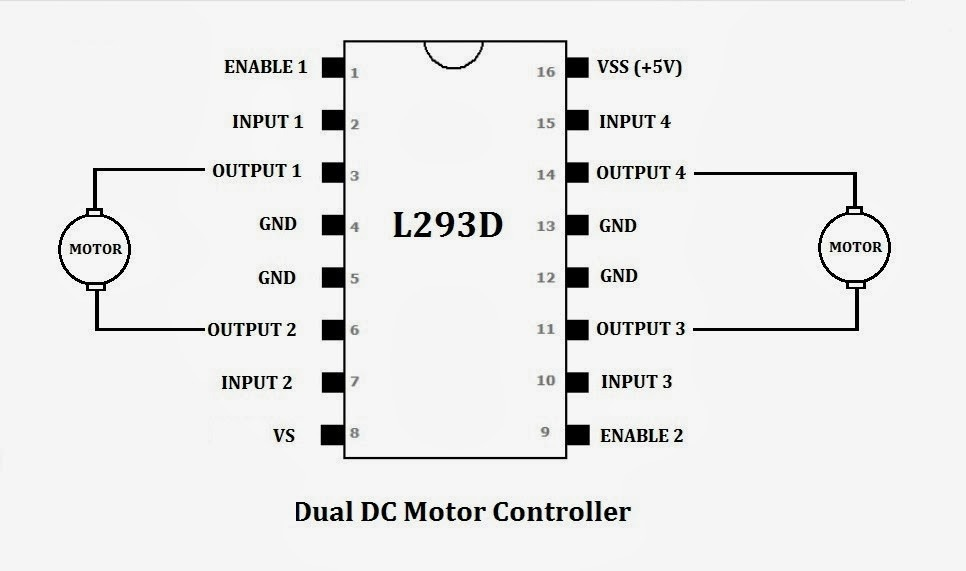
\includegraphics[width=0.7\linewidth]{informe_2/encapsulado_L293D}
	\caption{L293D}
	\label{fig:encapsuladol293d}
\end{figure}

\paragraph{}Al investigar sobre circuitos que provean puentes H para controlar motores de
continua, rápidamente encontramos el L293D. Este tiene 4 canales, cada uno
formando medio puente H. Dado que para girar motores en ambos sentidos se
requiere un puente completo, se pueden controlar dos motores con un solo
L293D.

En términos de conexionado provee un \emph{enable} por cada par de canales,
alimentación independiente para lógica y motores, y 6 pines centrales para
disipación de calor.

Respecto a la alimentación, requiere entre 4.5v y 30v. Dado el elevado consumo
es imposible alimentarlo directamente a través de la CIAA, por lo que se conecta  
de manera directa a la fuente de alimentación.

Soporta corrientes pico de 1.2A, por lo que es correcto colocar un disipador en
caso de que los motores consuman mucha corriente.

\subsubsection{Conexionado}

\paragraph{L293D}Las entradas de los L293D se controlan mediante PWM, permitiendo
controlar la velocidad de cada motor de manera independiente. Esto requiere
utilizar 8 PWM, dos para cada motor.

\subsubsection{Esquemático}

\begin{figure}[H]
	\centering
	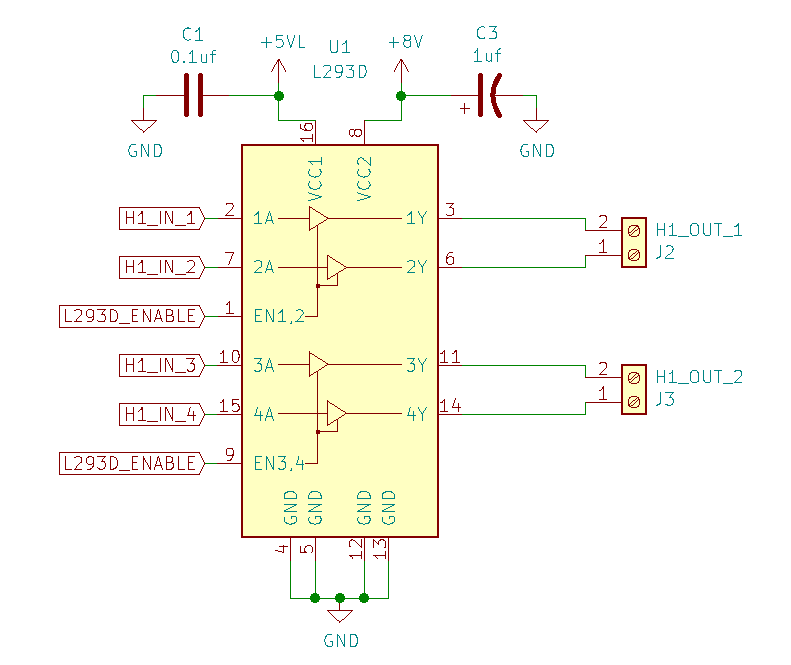
\includegraphics[width=0.7\linewidth]{informe_3/schem_L293D}
	\caption{Conexionado de un L293D}
	\label{fig:scheml293D}
\end{figure}

\paragraph{Capacitores} Se colocan capacitores en la alimentación según indica la hoja de datos del integrado L293D de Texas Instruments.

\subsection{Detector de Obstáculos}

\paragraph{} Para detectar obstáculos se utiliza el sensor de proximidad de Arduino
HC-SR04, que permite captar objetos entre 2cm y 400cm, con un ángulo de \ang{15}. 
Estos rangos resultan ideales para detectar obstáculos y actuar en consecuencia
en un vehículo a control remoto.

\subsubsection{Componentes a Utilizar}

\begin{longtable}[]{|c|c|c|c|p{3.2cm}|c|}
	\toprule
	Componente & Código & Valor & Cantidad & Función &
	Protocolo\tabularnewline
	\midrule
	\endhead
	Sensor Proximidad & HC-SR04 & - & 1 & Medir distancia a obstáculos &
	Digital\tabularnewline
	Buzzer & - & - & 1 & Indicar mediante sonido & Digital\tabularnewline
	\bottomrule
\end{longtable}

\subsubsection{Sensor de Proximidad}

\begin{figure}[H]
	\centering
	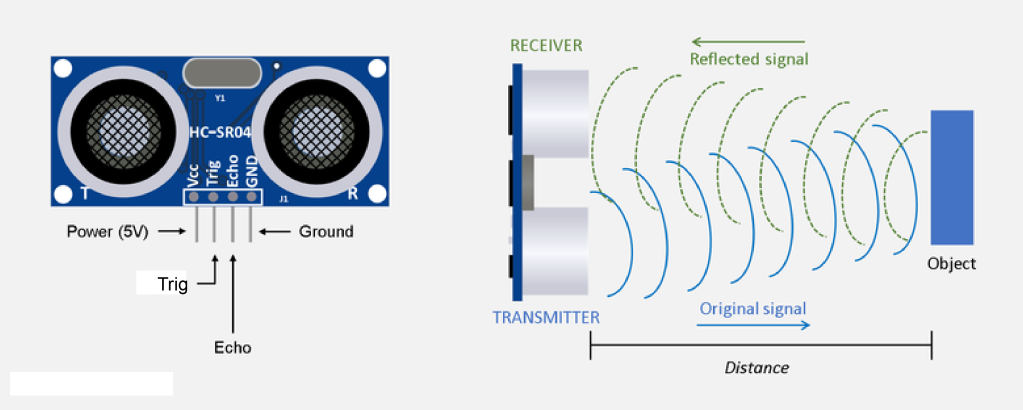
\includegraphics[width=0.7\linewidth]{informe_2/encapsulado_HC-SR04}
	\caption{HC-SR04}
	\label{fig:encapsuladohc-sr04}
\end{figure}

\paragraph{}El HC-SR04 es un sensor ultrasónico que permite calcular la distancia de los
objetos que se encuentran en frente a él, con un ángulo de visión de \ang{15}. 
Utiliza una onda sonora de 40kHz, inaudible para el oido humano, que se emite
cuando se coloca un 1 en el pin \emph{trigger}. Cuando el módulo detecta el rebote 
del pulso emitido, coloca un 1 en el pin \emph{echo}. Midiendo el tiempo entre la 
emisión del pulso y la recepción del eco, puede determinarse la distancia al objeto.

\subsubsection{Buzzer}
\paragraph{}Se utiliza como componente auxiliar para indicar la presencia de obstáculos mediante sonido.

\subsubsection{Conexionado}

\paragraph{HC-SR04} Dado que requiere medir con presición el tiempo transcurrido, es
necesario utilizar un timer en modo \emph{input capture} para lograr la
mayor presición posible. El \emph{trigger} se generará con una salida
GPIO común.

\paragraph{Buzzer}Dado que el consumo del buzzer supera el máximo tolerado por los puertos GPIO de la CIAA, 
se utiliza un transistor para alimentar el buzzer y asegurar su correcto funcionamiento
sin dañar ningún componente de hardware. Se utiliza el pin de GPIO7 como salida para el LED.

\subsubsection{Esquemático}

\begin{figure}[H]
	\centering
	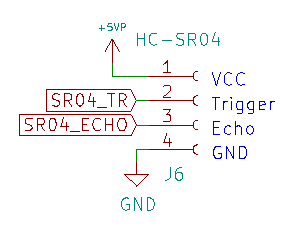
\includegraphics[width=0.4\linewidth]{informe_3/schem_hcsr04}
	\caption{Conexionado del HC-SR04}
	\label{fig:schemhcsr04}
\end{figure}

\begin{figure}[H]
	\centering
	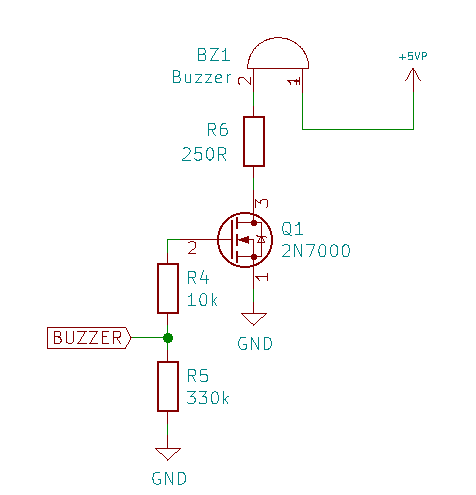
\includegraphics[width=0.5\linewidth]{informe_3/schem_buzzer}
	\caption{Conexionado del Buzzer}
	\label{fig:schembuzzer}
\end{figure}

\subsection{Indicadores de Estado}

\paragraph{}Se utiliza como componente auxiliar para indicar el estado del vehículo, un LED que indica si el vehículo está encendido.

\subsubsection{Esquemático}

\begin{figure}[H]
	\centering
	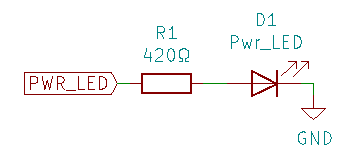
\includegraphics[width=0.4\linewidth]{informe_3/schem_pwr_led.png}
	\caption{Conexionado del LED de encendido}
	\label{fig:schempwrled}
\end{figure}

\section{Cálculos de Corriente}

\begin{longtable}[]{|c|c|c|}
	\toprule
	Subsistema & Tensión {[}V{]} & Corriente {[}mA{]}\tabularnewline
	\midrule
	\endhead
	Principal & 5 & 200\tabularnewline
	UART2 (BT) & - & 0.5\tabularnewline
	SCT * 3 & - & 0.16 *3\tabularnewline
	GPIO * 6 & - & 5 * 6\tabularnewline
	HM-10 & 5 & 10\tabularnewline
	L293D * 2 & 5 & 32 * 2\tabularnewline
	Motor * 4 & 8 & 100 * 4\tabularnewline
	------------- & ------------- & -----------------\tabularnewline
	\textbf{Total} & 5 & 280mA\tabularnewline
	\textbf{Total} & 8 & 400mA\tabularnewline
	\bottomrule
\end{longtable}

\paragraph{}Como se puede observar, dado la variedad de dispositivos y componentes,
se requieren dos valores de tensión diferentes. Además, al tratarse de un vehículo
manejado inalámbricamente, es necesario el uso de baterías. Utilizando dos baterías de Litio en serie 
se obtiene una tensión de entrada de aproximadamente 8V, por lo tanto, es necesario utilizar un conversor DC-DC 
step-down para obtener tensiones de 5V, y el conversor interno de la EDU-CIAA para obtener tension de de 3.3V.

Para alimentar la EDU-CIAA se opta por utilizar el conector Molex de alimentación externa, utilizando uno
igual en el poncho.

\subsubsection{Esquemático}

\begin{figure}[H]
	\centering
	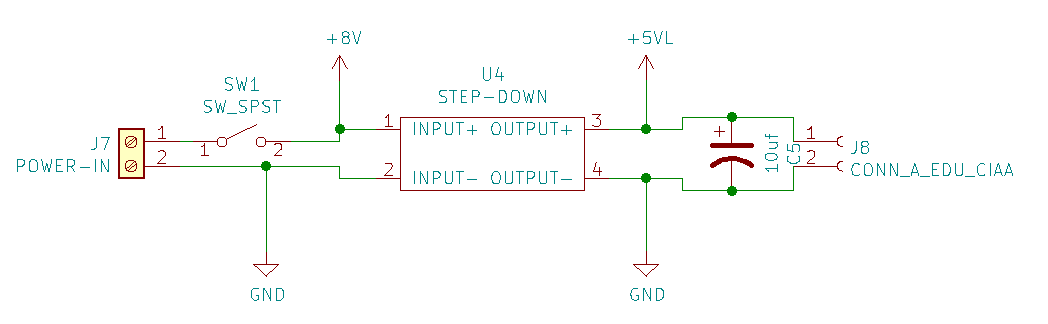
\includegraphics[width=0.8\linewidth]{informe_3/schem_fuente}
	\caption{Conexionado de la alimentación}
	\label{fig:schemfuente}
\end{figure}


\section{Diseño de PCB}

\paragraph{}Para el diseño de la PCB se tuvieron en cuenta las siguientes características:

\begin{itemize}
	\item Los conectores para los motores se deben disponer de manera que representen la rueda que está accionando.
	\item Los integrados L293D deben alejarse del resto de los componentes, ya que manejan una elevada corriente, y mucha temperatura.
	\item Los integrados L293D deben tener un plano de tierra en sus pines centrales, tal como indica  la hoja de datos, para poder disipar calor.
	\item El sensor ultrasonido HC-SR04 debe encontrarse en un extremo de la placa, de manera que la PCB pueda montarse con este sensor apuntando hacia adelante.
	\item El conector de baterías debe colocarse cerca de los extremos para no tener cables muy largos.
	\item El conector de alimentación para la EDU-CIAA debe encontrarse lo más cerca posible del conector en la EDU-CIAA.
	\item Tener en cuenta las recomendaciones de la cátedra respecto al ancho de pista, y distancia entre estas. Como así también el tamaño de los pads.
\end{itemize}

\subsection{Ancho de pistas}

\paragraph{} Además, debe tenerse en cuenta que dado el elevado consumo de los motores, es necesario tener en cuenta el ancho de las pistas, para no sobrecalentarlas. Utilizando la calculadora incorporada en KiCAD, se ve que una pista de 0.6mm (lo mínimo recomendado por la cátedra) puede tolerar sin problemas hasta 1.6A, por lo qué para todas las aplicaciones de GPIO, PWM, y alimentación de periféricos no hay problemas.

\paragraph{}Respecto a los L293D, están diseñados para soportar 300mA por canal, con una corriente máxima total de 1.2A, por lo qué, tanto las pistas de los motores como las de alimentación no requieren más que el ancho mínimo de 0.6mm. Sin embargo hay que tener en cuenta que el consumo de ambos combinados puede llegar a 2.4A, por lo que, la pista ``compartida'' de alimentación, si debe tener un ancho mayor, calculado en 1mm.

\paragraph{}El consumo total de la placa se estipula en 3A, dado que la CIAA consume alrededor de 200mA, y los motores 2.4A en los casos más extremos. Los consumos se resumen en la siguiente tabla:

\begin{longtable}[]{|c|c|c|c|}
	\toprule
	Pista & Consumo & Ancho real & Ancho a utilizar \tabularnewline
	\midrule
	Alimentación L293D & 1.3A & 0.4mm & 0.6mm \tabularnewline
	Alimentación de 2 L293D & 2.6A & 1mm & 1mm\tabularnewline
	8v (total) & 3A & 1.3mm & 1.3mm\tabularnewline
	5v & 0.4A & 0.08mm & 0.6mm\tabularnewline
	\endhead
	
	\bottomrule
\end{longtable}

Nota: para los cálculos finales, se agregó un 10\% de consumo por seguridad. Además, los cálculos para los L293D se realizan en base a las capacidades máximas de los mismos, y no con los motores que se disponen, que tienen un consumo mucho menor.

\subsection{Consideraciones para cada dispositivo}

Se trató de agrupar físicamente los componentes según su asociación lógica. Por ejemplo, las resistencias para un LED, cerca de ese LED.

\paragraph{L293D} Además de los requisitos mencionados previamente para los puentes H, debe tenerse en cuenta que requieren de capacitores filtro en las entradas de alimentación, cerca de cada integrado.

\subsection{BOM simplificado}

A continuación se presenta una versión simplificada de la lista de materiales en un formato legible, para un BOM más detallado que incluya las footprints de KiCAD, ver Anexo.


\begin{longtable}[]{|c|c|p{7cm}|}
	\toprule
	Referencia & Valor & Componente \tabularnewline
	\midrule
	\endhead
	
	BZ1 & - & Buzzer 12x9.5x7.6\tabularnewline
	C1 & 100nF & Capacitor cerámico\tabularnewline
	C2 & 100nF & Capacitor cerámico\tabularnewline
	C3 & 1uF & Capacitor electrolítico\tabularnewline
	C4 & 1uF & Capacitor electrolítico\tabularnewline
	C5 & 10uF & Capacitor electrolítico\tabularnewline
	D1 & LED 5mm & LED 5mm\tabularnewline
	D2 & LED 5mm & LED 5mm\tabularnewline
	D3 & LED 5mm & LED 5mm\tabularnewline
	J1 & Header HM10 & Tira de pin hembra x6\tabularnewline
	J2 & - & Bornera Azul de 2\tabularnewline
	J3 & - & Bornera Azul de 2\tabularnewline
	J4 & - & Bornera Azul de 2\tabularnewline
	J5 & - & Bornera Azul de 2\tabularnewline
	J6 & Header HC-SR04 & Tira de pin hembra x4\tabularnewline
	J7 & - & Bornera Azul de 2\tabularnewline
	J8 & - & Molex KK254 Macho 2 pines\tabularnewline
	Q1 & 2n7000 & Transistor 2n7000\tabularnewline
	R1 & 420R & Resistencia carbón 1/4\tabularnewline
	R2 & 420R & Resistencia carbón 1/4\tabularnewline
	R3 & 420R & Resistencia carbón 1/4\tabularnewline
	R4 & 10k & Resistencia carbón 1/4\tabularnewline
	R5 & 330k & Resistencia carbón 1/4\tabularnewline
	R6 & 250R & Resistencia carbón 1/4\tabularnewline
	SW1 & Switch SPST & Interruptor DIP 1 posición\tabularnewline
	U1 & L293D & Puente H L293D\tabularnewline
	U2 & L293D & Puente H L293D\tabularnewline
	U4 & Mini360 & Fuente Step-Down mini360\tabularnewline
	X & Pines & Tira de pines p/edu-ciaa\tabularnewline
	N/A & HM-10 & HM-10\tabularnewline
	N/A & HC-SR04 & HC-SR04\tabularnewline	
	
	\bottomrule
\end{longtable}
